\section{Getting a Pixel's Offset}\label{ssc:xy_angles}
In \cref{ch:obj_rec} a basis for object recognition was presented which is used to identify a target that the system are tracking. Using object recognition the pixel which is the center of the target can be obtained. This pixel's position in an image is used to calculate the difference between the direction of a vector with base in the lens' centre and direction of the object. Figure \ref{fig:calculating_angles} illustrates an image where a pixel is used as identifier of the object. Two coordinate systems are defined on the image in order to obtain this direction, the first system has the axes $Offset_x$ and $Offset_y$ which are used to tell a pixel's position ont he image. The other coordinate system's origin is in the centre of the image and is used to define a vector with the tail placed in the camera's lens' centre. This vector is adjusted to point towards the intended object.

\begin{figure}[ht]
    \centering
    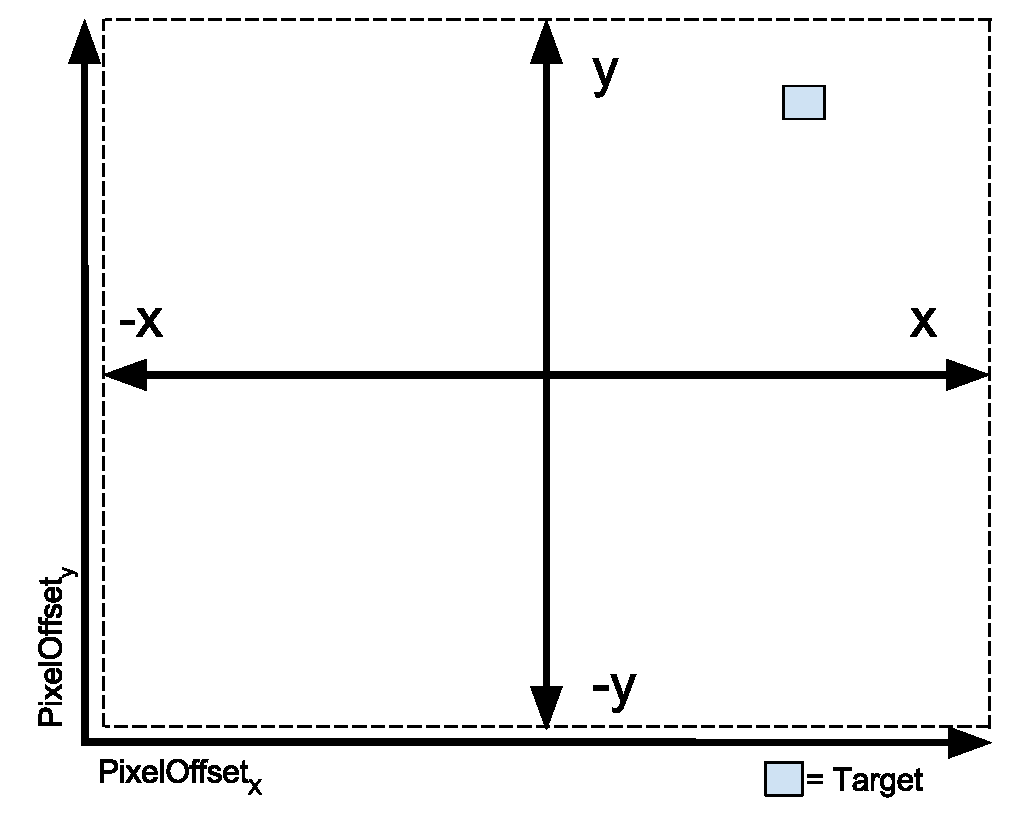
\includegraphics[scale=0.65]{graphics/signed_angles_simple.eps}
    \caption{Example with a marked centre and a target in top right quadrant}
    \label{fig:calculating_angles}
\end{figure}

Using the definition of the x- and y-axis from the image, the z-axis in the 3D room will also have origin in the centre of the lens, but the depth of the image will follow the negative z-axis, resulting in the vector, with tail in the lens, to be defined as
$\left[\!\begin{array}{c}
0\\
0\\
-1
\end{array}\!\right] $
since the vector's direction is away from the lens along the negative z-axis. Before adjusting this vector the deviation along the y- and x-axis must be found. The deviation is found by calculating the fraction of how much the object's pixel is along the two axes. The equations for this are:
\begin{equation}
\frac{Offset_X - 0.5 * Width}{0.5 * Width} \label{eq:offset-x}
\end{equation}
\begin{equation}
\frac{Offset_Y - 0.5 * Height}{0.5 * Height} \label{eq:offset-y}
\end{equation}
\Cref{eq:offset-x} and \cref{eq:offset-y} show the fraction of how far the pixel is along the x- and y-axis, respectively. With the knowledge of these offsets it is possible to calculate the angles for which the vector shall be rotated. A camera has one \acrfull{fov} for each axis. The angles of these \glspl{fov} are used to calculate how many degrees the pixel has moved along the axes. The \gls{fov} is included in \cref{eq:offset-x_fov} and \cref{eq:offset-y_fov}, as $F_x$ for the horizontal \gls{fov} and $F_y$ for the vertical \gls{fov}. Furthermore, the \gls{fov} is halved because the angles are found relative to the centre.

\begin{equation}
\frac{Offset_X - 0.5 * Width}{0.5 * Width}*F_x*0.5 \label{eq:offset-x_fov}
\end{equation}
\begin{align}
\frac{Offset_Y - 0.5 * Height}{0.5 * Height}*F_y*0.5 \label{eq:offset-y_fov}
\end{align}

\Cref{eq:offset-x_fov} and \cref{eq:offset-y_fov} are the final equations that are used for the calculations of the angles. The following section will focus on the rotation of matrices around the x- and y-axes. Lastly an example is given to illustrate the use of the techniques.